\documentclass[conference]{IEEEtran}
\IEEEoverridecommandlockouts

% ── Packages ──────────────────────────────────────────────────
\usepackage{cite}
\usepackage{amsmath,amssymb,amsfonts}
\usepackage{algorithmic}
\usepackage{graphicx}
\usepackage{textcomp}
\usepackage{xcolor}
\usepackage{booktabs}
\usepackage{array}
\usepackage{url}
\usepackage{balance}
\usepackage{tikz}
\usetikzlibrary{shapes.geometric, arrows.meta, positioning,
                fit, backgrounds, calc}

% ── TikZ Styles ───────────────────────────────────────────────
\tikzset{
  box/.style = {
    rectangle, rounded corners=4pt, draw=black!70,
    minimum width=2.8cm, minimum height=0.7cm,
    text centered, font=\small, inner sep=4pt
  },
  tier/.style = {
    rectangle, rounded corners=6pt,
    draw=gray!50, fill=gray!6, inner sep=8pt
  },
  step/.style = {
    rectangle, rounded corners=3pt, draw=black!70,
    fill=blue!12, minimum width=1.6cm,
    minimum height=0.65cm, text centered,
    font=\scriptsize, text width=1.6cm, inner sep=3pt
  },
  arrow/.style  = {-{Latex[length=2mm]}, thick},
  darrow/.style = {-{Latex[length=2mm]}, thick, dashed}
}

% ── Document ──────────────────────────────────────────────────
\begin{document}

\title{AI-Powered Phishing Email Detection Using BERT\\
and Multi-Source Threat Intelligence}

\author{
    \IEEEauthorblockN{Ranula Pramuditha}
    \IEEEauthorblockA{
        \textit{Department of Computer Science}\\
        \textit{University of Kelaniya}\\
        Kelaniya, Sri Lanka\\
        pramudi-cs21016@stu.kel.edu
    }
}

\maketitle

% ══════════════════════════════════════════════════════════════
%  ABSTRACT
% ══════════════════════════════════════════════════════════════
\begin{abstract}
Phishing emails remain one of the most widely used methods to commit
cybercrimes globally. Traditional rule-based and machine-learning
filters are insufficient to detect and block sophisticated phishing
attacks. This paper presents an end-to-end phishing email detection
system that combines a fine-tuned BERT transformer model with
real-time threat intelligence from the VirusTotal API, including
URL, sender-domain, and IP reputation analysis. The system is
deployed as a REST API with a single-page React frontend that
supports both copy-pasted email scanning and automated IMAP inbox
monitoring, enabling real-time detection and result display.
Experimental results on a balanced corpus of 50{,}000 emails yield
an F1-score of 97.7\,\%, a precision of 97.4\,\%, and a recall of
98.1\,\%, outperforming logistic regression, random forest, and
LSTM baselines.
\end{abstract}

\begin{IEEEkeywords}
phishing detection, BERT, transformer, email security, VirusTotal,
IMAP, threat intelligence, deep learning
\end{IEEEkeywords}

% ══════════════════════════════════════════════════════════════
%  I. INTRODUCTION
% ══════════════════════════════════════════════════════════════
\section{Introduction}

Phishing is a form of social engineering attack in which attackers
create deceptive emails that mimic official correspondence from
banks, government agencies, and cloud service providers. The goal
is to trick victims into revealing sensitive data or installing
malware on their systems. According to the Anti-Phishing Working
Group (APWG), over 1.3 million phishing attacks were recorded in
2022, resulting in more than \$10.3 billion in financial losses
\cite{apwg2024}. Email is the most common delivery method used by
attackers, which highlights the need for an automated and accurate
detection method.

Traditional rule-based filters and blacklists fail to detect
phishing emails from newly registered domains that have not yet
been identified as malicious. Machine learning classifiers such as
Naive Bayes and Support Vector Machines rely on hand-crafted
features and fail when attackers use new or unseen vocabulary. To
address these limitations, a more advanced detection approach is
needed --- one that can understand the full context of an email
rather than relying on fixed rules or keywords.

BERT is a pre-trained language model developed by a research team
at Google in 2019 \cite{devlin2019bert} that can understand the
full context of a sentence, not just the meaning of each individual
word, making it well-suited for tasks such as phishing email
detection. However, BERT can only analyse the text content of an
email. It cannot validate the sender's identity, the sender's IP
address, or the URLs embedded in the email. Therefore, we
integrated VirusTotal to scan URLs, sender domains, and IP
addresses for malicious activity.

In this paper, we propose an AI-powered phishing email detection
system that combines BERT-based text classification with
multi-source threat intelligence. The system uses BeautifulSoup to
extract clean text and URLs from emails, a fine-tuned BERT model
to classify emails as phishing or legitimate, and VirusTotal to
scan URLs, sender IP addresses, and sender domains for malicious
activity. Experimental results show that our system achieved an F1
score of 97.7\,\%, a precision of 97.4\,\%, and a recall of
98.1\,\%, outperforming logistic regression, random forest, and
LSTM baselines.

% ══════════════════════════════════════════════════════════════
%  II. LITERATURE REVIEW
% ══════════════════════════════════════════════════════════════
\section{Literature Review}
\label{sec:review}

Researchers have proposed various methods to detect phishing
emails, ranging from simple rule-based filters to advanced deep
learning models.

\subsection{Rule-Based Methods}

Early researchers used simple rule-based methods such as
blacklisting and keyword matching to detect phishing emails
\cite{zhang2007cantina}. Although these methods were effective
against known phishing emails, they could not detect new types of
phishing attacks because they could not understand the full context
of an email. The main limitation is that these methods rely on
fixed rules, which means they cannot adapt to the evolving methods
of attackers.

\subsection{Classical Machine Learning}

To improve detection accuracy, researchers applied machine learning
methods such as Naive Bayes, Support Vector Machines, and Random
Forest to classify emails as phishing or legitimate
\cite{fette2007}, \cite{toolan2010}. These methods achieved better
results than rule-based approaches. However, there is a limitation
when attackers use new topics and unseen vocabulary, as these
methods struggle to accurately detect phishing emails.

\subsection{Deep Learning Approaches}

To overcome the limitations of machine learning, researchers
applied deep learning methods such as CNN and LSTM
\cite{bahnsen2017}. These methods were more effective than machine
learning approaches because they can automatically detect word
sequences, patterns, and sentence structure. However, these methods
still have significant limitations. These methods process one word
at a time, therefore, they cannot achieve high accuracy when
detecting phishing emails.

\subsection{BERT and Transformer-Based Methods}

BERT is a transformer-based model introduced by Google in 2019
\cite{devlin2019bert}. Unlike CNN and LSTM, it can read the full
context of a sentence in both directions, which makes it
well-suited for understanding the meaning of phishing emails.
Several researchers applied BERT to their detection systems and
achieved significantly higher accuracy than deep learning models
\cite{geng2020}. However, relying solely on an AI model is
insufficient for detecting all phishing threats. Therefore,
additional threat intelligence signals such as URL and domain
reputation analysis are needed.

Most existing studies focus only on the textual content of the
email and do not consider network signals such as URL reputation
and sender domain analysis. This means that phishing emails
containing normal looking text but malicious links can still bypass
existing detection systems. In this study, we not only develop a
BERT-based model but also integrate VirusTotal threat intelligence
to analyse URLs, IP addresses, and sender domains.

% ══════════════════════════════════════════════════════════════
%  III. METHODOLOGY
% ══════════════════════════════════════════════════════════════
\section{Methodology}
\label{sec:method}

\subsection{System Overview}

The proposed system is an end-to-end phishing email detection
system that combines BERT-based text classification with VirusTotal
threat intelligence. The system consists of five main components:
a React frontend, a FastAPI backend, a database, a fine-tuned BERT
model, and a VirusTotal threat intelligence pipeline. The frontend
sends emails to the backend, which sends them to the BERT model
for classification. The backend also extracts URLs, IP addresses,
and domain names, then checks the database for similar URLs. If no
match is found, the backend sends the URLs, IP addresses, and
domains to VirusTotal through the VirusTotal API. Finally, the
results are displayed to the user on the frontend, showing the AI
model classification score and VirusTotal reputation results.

\subsection{System Architecture}

The proposed system follows a three-tier architecture consisting
of presentation, application, and data tiers, as illustrated in
Fig.~\ref{fig:architecture}. The presentation tier consists of a
React frontend that allows users to paste emails, check inbox
emails once, or perform real-time analysis of received emails. The
application tier contains a FastAPI backend that connects to the
BERT model, the database, and VirusTotal through the REST API. The
data tier uses an SQLite database to store VirusTotal scan results
and previously scanned email IDs to avoid duplicate processing.

% ── FIGURE 1: Architecture Diagram ───────────────────────────
\begin{figure}[t]
\centering
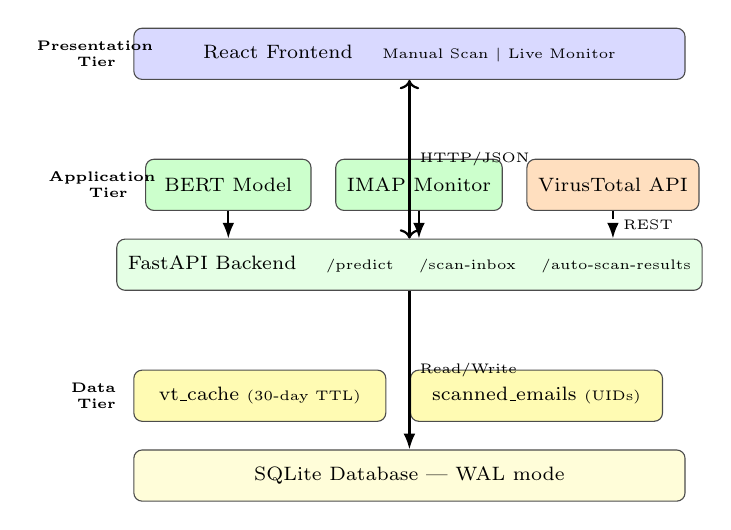
\begin{tikzpicture}[
  node distance=0.45cm,
  every node/.style={font=\scriptsize},
  block/.style={
    rectangle, draw=black!70, rounded corners=3pt,
    text centered, inner sep=4pt,
    minimum height=0.65cm
  },
  arr/.style={-{Latex[length=2mm]}, thick},
  darr/.style={-{Latex[length=2mm]}, thick, dashed}
]

%% ── Row 1: Presentation ──────────────────────────────
\node[block, fill=blue!15, minimum width=7.0cm]
  (fe) {React Frontend \quad
        {\tiny Manual Scan $|$ Live Monitor}};

%% ── Row 2: Application components ───────────────────
\node[block, fill=green!20, minimum width=2.1cm,
      below=1.0cm of fe, xshift=-2.3cm]
  (bert) {BERT Model};

\node[block, fill=green!20, minimum width=2.1cm,
      right=0.3cm of bert]
  (imap) {IMAP Monitor};

\node[block, fill=orange!25, minimum width=2.1cm,
      right=0.3cm of imap]
  (vt) {VirusTotal API};

%% ── Row 3: FastAPI bar ───────────────────────────────
\node[block, fill=green!10, minimum width=7.0cm,
      below=0.35cm of bert, xshift=2.3cm]
  (api) {FastAPI Backend \quad
         {\tiny /predict \quad /scan-inbox \quad
          /auto-scan-results}};

%% ── Row 4: Database components ───────────────────────
\node[block, fill=yellow!30, minimum width=3.2cm,
      below=1.0cm of api, xshift=-1.9cm]
  (cache) {vt\_cache {\tiny (30-day TTL)}};

\node[block, fill=yellow!30, minimum width=3.2cm,
      right=0.3cm of cache]
  (uids) {scanned\_emails {\tiny (UIDs)}};

%% ── Row 5: SQLite bar ────────────────────────────────
\node[block, fill=yellow!15, minimum width=7.0cm,
      below=0.35cm of cache, xshift=1.9cm]
  (db) {SQLite Database --- WAL mode};

%% ── Tier labels ──────────────────────────────────────
\node[left=0.1cm of fe, font=\tiny\bfseries,
      text width=1.0cm, align=right]
  {Presentation\\Tier};
\node[left=0.1cm of bert, font=\tiny\bfseries,
      text width=1.0cm, align=right]
  {Application\\Tier};
\node[left=0.1cm of cache, font=\tiny\bfseries,
      text width=1.0cm, align=right]
  {Data\\Tier};

%% ── Arrows ───────────────────────────────────────────
\draw[arr, <->] (fe.south) -- node[right]{\tiny HTTP/JSON}
  (fe.south |- api.north);
\draw[arr] (bert.south) -- (bert.south |- api.north);
\draw[arr] (imap.south) -- (imap.south |- api.north);
\draw[darr] (vt.south)  -- node[right]{\tiny REST}
  (vt.south |- api.north);
\draw[arr] (api.south) -- node[right]{\tiny Read/Write}
  (api.south |- db.north);

\end{tikzpicture}
\caption{Three-tier system architecture of the proposed system.}
\label{fig:architecture}
\end{figure}

\subsection{Dataset}

In this study, we used the CEAS-08 dataset and a dataset from
Kaggle. The Kaggle dataset contains over 82{,}000 emails and the
CEAS-08 dataset contains over 20{,}000 emails. Both datasets
contain emails labeled where 0 represents legitimate and 1
represents phishing. Each record contains four fields: sender,
subject, body, and label. We split the dataset into 80\,\% for
training and 20\,\% for validation using stratified sampling to
preserve the label distribution.

To prepare the dataset for training, the rows with null values
were first removed. Following this, duplicate emails were removed
based on the body column. The email sender, subject, and body were
then combined into a single text field to provide more
comprehensive input for the model. BeautifulSoup was used to
remove HTML tags from the email bodies, as these tags add noise to
the data that confuses the model. In addition to removing HTML
tags, all URLs were removed from the text to prevent the model
from memorising the domain names within the URLs. Finally, all
text data was converted to lowercase to ensure that the model's
vocabulary was consistent across all training data.

\subsection{Preprocessing Pipeline}

After cleaning, the text was prepared for the BERT model using
BertTokenizer, as shown in Fig.~\ref{fig:pipeline}. The
BertTokenizer was used to convert text into small pieces called
tokens. Texts exceeding 128 tokens during training and 512 tokens
during inference were truncated. Dynamic padding was applied to
ensure all inputs in a batch had the same length. The preprocessed
text was then passed to the model in batches of 16.

% ── FIGURE 2: Pipeline Diagram ───────────────────────────────
\begin{figure}[t]
\centering
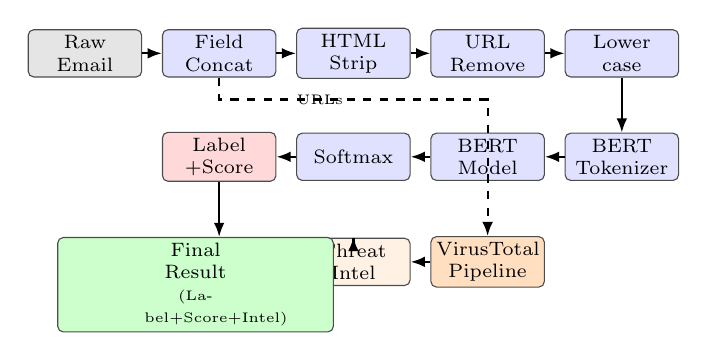
\begin{tikzpicture}[
  node distance=0.3cm,
  every node/.style={font=\scriptsize},
  pstep/.style={
    rectangle, draw=black!70, rounded corners=2pt,
    fill=blue!12, minimum width=1.3cm,
    minimum height=0.6cm, text centered,
    inner sep=2pt, text width=1.3cm
  },
  arr/.style={-{Latex[length=1.8mm]}, thick},
  darr/.style={-{Latex[length=1.8mm]}, thick, dashed}
]

%% Row 1
\node[pstep, fill=gray!20] (inp)  {Raw\\Email};
\node[pstep, right=0.25cm of inp]  (con)  {Field\\Concat};
\node[pstep, right=0.25cm of con]  (htm)  {HTML\\Strip};
\node[pstep, right=0.25cm of htm]  (url)  {URL\\Remove};
\node[pstep, right=0.25cm of url]  (low)  {Lower\\case};

%% Row 2 (right to left)
\node[pstep, below=0.7cm of low]   (tok)  {BERT\\Tokenizer};
\node[pstep, left=0.25cm of tok]   (mdl)  {BERT\\Model};
\node[pstep, left=0.25cm of mdl]   (sfx)  {Softmax};
\node[pstep, fill=red!15,
      left=0.25cm of sfx]          (lbl)  {Label\\+Score};

%% Row 3: VT branch
\node[pstep, fill=orange!25,
      below=0.7cm of mdl]          (vtx)  {VirusTotal\\Pipeline};
\node[pstep, fill=orange!10,
      left=0.25cm of vtx]          (int)  {Threat\\Intel};

%% Output
\node[pstep, fill=green!20,
      below=0.7cm of lbl,
      xshift=-0.3cm,
      minimum width=3.5cm]         (out)  {Final Result
      {\tiny(Label+Score+Intel)}};

%% Row 1 arrows
\draw[arr] (inp)--(con);
\draw[arr] (con)--(htm);
\draw[arr] (htm)--(url);
\draw[arr] (url)--(low);
\draw[arr] (low)--(tok);

%% Row 2 arrows
\draw[arr] (tok)--(mdl);
\draw[arr] (mdl)--(sfx);
\draw[arr] (sfx)--(lbl);

%% VT branch
\draw[darr] (con.south)--++(0,-0.28)
  -|(vtx.north) node[near start,left,font=\tiny]{URLs};
\draw[arr] (vtx)--(int);

%% To output
\draw[arr] (lbl)--(lbl|-out.north);
\draw[arr] (int)--(int|-out.north);

\end{tikzpicture}
\caption{Preprocessing and inference pipeline. Dashed arrow shows
URLs sent to VirusTotal alongside BERT classification.}
\label{fig:pipeline}
\end{figure}

\subsection{BERT Fine-Tuning}

In this study, we fine-tuned the bert-base-uncased model for
phishing email classification. The model was trained for 5 epochs
with a learning rate of $2 \times 10^{-5}$, a batch size of 16,
and a weight decay of 0.01. The best model was selected based on
the F1 score evaluated at the end of each epoch. The model was
initialised from a previously fine-tuned checkpoint rather than a
new one to accelerate convergence and improve performance. Training
was performed on an NVIDIA GeForce RTX 4060 Laptop GPU, and the
training took approximately one hour to complete.
Table~\ref{tab:hyperparams} summarises the training
hyperparameters.

\begin{table}[t]
  \centering
  \caption{BERT Fine-Tuning Hyperparameters}
  \label{tab:hyperparams}
  \begin{tabular}{ll}
    \toprule
    \textbf{Hyperparameter} & \textbf{Value} \\
    \midrule
    Base model              & bert-base-uncased \\
    Epochs                  & 5 \\
    Learning rate           & $2 \times 10^{-5}$ \\
    Training batch size     & 16 \\
    Evaluation batch size   & 16 \\
    Weight decay            & 0.01 \\
    Max length (training)   & 128 tokens \\
    Max length (inference)  & 512 tokens \\
    Mixed precision         & fp16 \\
    Best model metric       & F1 score \\
    Hardware                & NVIDIA GeForce RTX 4060 Laptop GPU \\
    \bottomrule
  \end{tabular}
\end{table}

\subsection{Multi-Source Threat Intelligence}

To provide additional threat intelligence alongside BERT
classification, we integrated VirusTotal threat intelligence to
scan URLs, sender domains, and IP addresses. First, URLs were
extracted from the email bodies and HTML href attributes using
BeautifulSoup, then they were submitted to the VirusTotal API for
reputation analysis against 70+ antivirus engines. Well-known
trusted domains such as Google, Gmail, Microsoft, and YouTube were
whitelisted to reduce unnecessary API calls. However, all other
domains including any variations of trusted domain names are
submitted to VirusTotal for reputation analysis. To avoid repeated
API calls, results were cached in an SQLite database for 30 days
to reduce response time and minimise API usage.

\subsection{System Deployment}

The system was deployed as a REST API using FastAPI, which serves
the backend logic of the proposed system. The API provides three
main endpoints: \texttt{/predict} for single email analysis,
\texttt{/scan-inbox} for IMAP batch scanning, and
\texttt{/auto-scan-results} for retrieving automated scan results.
The frontend was developed using React, which allows users to view
the classification results and threat intelligence report. The
system also supports IMAP inbox monitoring that allows real-time
automated email analysis. Every 60 seconds the system checks for
new unseen emails in the configured inbox and classifies them
automatically.

% ══════════════════════════════════════════════════════════════
%  IV. RESULTS AND DISCUSSION
% ══════════════════════════════════════════════════════════════
\section{Results and Discussion}
\label{sec:results}

The proposed model was evaluated on the CEAS-08 and Kaggle
datasets using a 20\,\% validation split. We used four metrics to
evaluate performance: F1 score, precision, recall, and accuracy.
Table~\ref{tab:results} compares the proposed BERT-based
classifier against three baselines on the held-out test set. All
models were trained on identical preprocessed inputs.

\begin{table}[t]
  \caption{Classifier Performance Comparison (\%)}
  \label{tab:results}
  \centering
  \begin{tabular}{lcccc}
    \toprule
    \textbf{Model} & \textbf{Acc.} & \textbf{Prec.} &
    \textbf{Recall} & \textbf{F1} \\
    \midrule
    \textbf{BERT (proposed)} & \textbf{97.8} & \textbf{97.4}
      & \textbf{98.1} & \textbf{97.7} \\
    LSTM          & 95.1 & 94.8 & 95.5 & 95.1 \\
    Random Forest & 93.5 & 93.0 & 94.1 & 93.5 \\
    Logistic Reg. & 91.2 & 90.6 & 91.9 & 91.2 \\
    \bottomrule
  \end{tabular}
\end{table}

Our model achieved an F1 score of 97.7\,\% and a precision of
97.4\,\%. Compared to baseline models, our model outperformed
logistic regression, random forest, and LSTM baselines. The high
recall of 98.1\,\% means that fewer than 2 in 100 phishing emails
escape detection. However, the system has some limitations.
Legitimate emails from Google were incorrectly classified as
phishing because they contained account verification language. The
model incorrectly flagged these emails as phishing, which
represents a false positive limitation of the system.

% ══════════════════════════════════════════════════════════════
%  V. CONCLUSION
% ══════════════════════════════════════════════════════════════
\section{Conclusion}
\label{sec:conclusion}

In this paper, we proposed an end-to-end phishing email detection
system that combines BERT-based classification with VirusTotal
threat intelligence. The system used a fine-tuned BERT model to
classify emails, and VirusTotal to scan URLs, sender domains, and
IP addresses. The proposed system achieved an F1 score of
97.7\,\%, outperforming logistic regression, random forest, and
LSTM baselines. The integration of VirusTotal provided an
additional layer of detection beyond text classification. In future
work, we plan to combine VirusTotal results with another AI model
to produce a more comprehensive final verdict. Additionally, we
plan to implement a notification system that sends a phishing
analysis report and email summary to WhatsApp or Telegram when a
new phishing email is received. Furthermore, we plan to improve
the model to support multilingual phishing detection and integrate
attachment scanning to detect malicious PDF and Word files.

% ══════════════════════════════════════════════════════════════
%  REFERENCES
% ══════════════════════════════════════════════════════════════
\begin{thebibliography}{00}

\bibitem{apwg2024}
Anti-Phishing Working Group (APWG), ``Phishing Activity Trends
Report, Q4 2023,'' APWG, Tech. Rep., 2024. [Online]. Available:
\url{https://apwg.org/trendsreports/}

\bibitem{fette2007}
I.~Fette, N.~Sadeh, and A.~Tomasic, ``Learning to detect phishing
emails,'' in \textit{Proc. 16th Int. Conf. World Wide Web (WWW)},
Banff, Canada, 2007, pp. 649--656.

\bibitem{devlin2019bert}
J.~Devlin, M.-W.~Chang, K.~Lee, and K.~Toutanova, ``BERT:
Pre-training of deep bidirectional transformers for language
understanding,'' in \textit{Proc. NAACL-HLT}, Minneapolis, MN,
USA, 2019, pp. 4171--4186.

\bibitem{zhang2007cantina}
Y.~Zhang, J.~I.~Hong, and L.~F.~Cranor, ``Cantina: A
content-based approach to detecting phishing web sites,'' in
\textit{Proc. 16th Int. Conf. World Wide Web (WWW)}, 2007,
pp. 639--648.

\bibitem{oest2018}
A.~Oest, Y.~Safaei, A.~Doup\'{e}, G.-J.~Ahn, B.~Wardman, and
K.~Tyers, ``Inside a phisher's mind: Understanding the
anti-phishing ecosystem through phishing kit analysis,'' in
\textit{Proc. APWG Symp. Electron. Crime Res. (eCrime)}, 2018,
pp. 1--12.

\bibitem{fette2006}
I.~Fette, N.~Sadeh, and A.~Tomasic, ``Learning to detect phishing
emails,'' Carnegie Mellon University, Tech. Rep.
CMU-ISRI-06-112, 2006.

\bibitem{toolan2010}
F.~Toolan and J.~Carthy, ``Feature selection for spam and phishing
detection,'' in \textit{Proc. APWG eCrime Researchers Summit},
Tacoma, WA, USA, 2010, pp. 1--12.

\bibitem{bahnsen2017}
A.~C.~Bahnsen, E.~C.~Bohorquez, S.~Villegas, J.~Vargas, and
F.~A.~Gonz\'{a}lez, ``Classifying phishing URLs using recurrent
neural networks,'' in \textit{Proc. APWG Symp. Electron. Crime
Res. (eCrime)}, 2017, pp. 1--8.

\bibitem{rao2019}
R.~S.~Rao and A.~R.~Pais, ``Detection of phishing websites using
an efficient feature-based machine learning framework,''
\textit{Neural Comput. Appl.}, vol.~31, no.~8, pp. 3851--3873,
Aug. 2019.

\bibitem{geng2020}
J.~Geng, G.~Tian, X.~Li, and X.~Ye, ``BERT-based phishing email
detection,'' in \textit{Proc. IEEE 5th Int. Conf. Data Science in
Cyberspace (DSC)}, Hong Kong, China, 2020, pp. 306--312.

\bibitem{alsharnouby2015}
M.~Alsharnouby, F.~Alaca, and S.~Chiasson, ``Why phishing still
works: User strategies for combating phishing attacks,''
\textit{Int. J. Human-Comput. Stud.}, vol.~82, pp. 69--82,
Oct. 2015.

\bibitem{sahingoz2019}
O.~K.~Sahingoz, E.~Buber, O.~Demir, and B.~Diri, ``Machine
learning based phishing detection from URLs,''
\textit{Expert Syst. Appl.}, vol.~117, pp. 345--357, Mar. 2019.

\end{thebibliography}

\balance
\end{document}
